\subsubsection*{Task} 
Check what types of indexes does Your DBMS support. Name and describe those of them which are especially useful for speeding up Your
queries.\newline

\noindent Oracle 10g provides several indexing schemes
\footnote{\url{http://docs.oracle.com/cd/B19306_01/server.102/b14231/indexes.htm}}
that provide complementary performance functionality. These are:
\begin{itemize}
\item B-tree indexes: the default and the most common
\item B-tree cluster indexes: defined specifically for cluster
\item Hash cluster indexes: defined specifically for a hash cluster
\item Global and local indexes: relate to partitioned tables and indexes
\item Reverse key indexes: most useful for Oracle Real Application Clusters applications
\item Bitmap indexes: compact; work best for columns with a small set of values
\item Function-based indexes: contain the precomputed value of a function/expression
\item Domain indexes: specific to an application or cartridge.
\end{itemize}

A B-tree is a tree data structure that keeps data sorted and allows searches, sequential access, insertions, and deletions in logarithmic time.\footnote{\url{http://en.wikipedia.org/wiki/B-tree}} It is designed to allow quickly finding those tuples that have a specific key value. For this reason, they are suitable for speeding up selection operations.\footnote{Data Warehouse Design: Modern Principles and Methologies, section 11.2.1}

We will use B-trees to index primary keys and other columns which are used to filter data.

Bitmap indexes are also designed for finding tuples by a specific key but are very structurally different from B-tree indexes. A bitmap index is like two-dimensional boolean arrays of the same size as the number of rows for every value where each element contains a binary value indicating whether the row contains this value. In this structure, the binary value takes up only 1 bit and for each possible value the number of rows bits are used. It is much more space efficient than B-trees if the number of possible values is very low. Another feature of bitmap indexes is the ability to quickly do index intersections.

In our data warehouse we have several columns which contain only a small set of possible values. By using bitmap indexes for these columns, it is possible to reduce the storage space taken up by the indexes. When a query filters data with several of these columns at the same time, the database system will combine these indexes to return data very quickly.


\subsection*{Task} 
For the chosen queries and their versions which use the materialized views,
implement indexes to improve their performance (You can try to evaluate
several strategies and choose the best one, e.g. best speed/size ratio).
Argue Your choice. Describe the overhead (index size, computation time,
index update costs, etc.) of implementing the chosen indexes.\newline

\noindent The following formulas to calculate the size of indexes are used\footnote{Data Warehouse Design: Modern Principles and Methologies, section 11.2.1}: 
\begin{itemize}
    \item B-Tree index: $(NK*len(k)+NR*len(r))/(D*u)$ \footnote{
Shortcuts used: $NK$ = number of distinct key values, NR = 1000000 number of relations, len(k) = 8 = key length in kilobytes, len(r) = 8 = RID (disk page and location) length in kilobytes, D = 4096 disk page size in kilobytes, u = 1 fill factor for leaves}
    \item Bitmap index: $(NR/D*8)*NK$
\end{itemize}

\subsection*{Subscription revenue by country} 
\begin{lstlisting}[language=sql]
select l.country, sum(price * (1-discount) * quantity) revenue, 
  sum(quantity) subscriptions 
from sub_subscription s 
join sub_location l on s.keylocation = l.keylocation 
join sub_date d on s.keydate = d.keydate and d.year = 2010
group by l.country 
order by revenue desc
\end{lstlisting}

There should be B-tree indexes $sub\_subscription(keyLocation)$, $sub\_location(keyLocation)$, $sub\_subscription(keyDate)$, $sub\_date(keyDate)$ to avoid a full table scan when joining two tables. 
Bitmap indexes are not suitable for this since there are many possible values and such a bitmap index would take up much more space. Assuming 1 million distinct tuples, the B-tree index size would be 21.48 MB (vs 30.52 GB for bitmap indexes). In a B-tree index for every tuple insertion time complexity is $O(log(n))$\footnote{\url{http://en.wikipedia.org/wiki/B-tree}}

There should be an index $sub\_date(year)$ so that it can be used when data is filtered by year. Assuming 365 days per year and 100 years $\rightarrow$ 36500 tuples. Assuming the total number of distinct values is 100 (covering 100 years), it is reasonable to consider bitmap indexes for this index. A bitmap index would take up 7.129 MB, while a B-tree index would take up 0.07 MB of disk space. While a bitmap index has a 100x larger space overhead, it is negligible on modern systems. Considering the fact that other columns of the table $sub\_date$ are perfect candidates for bitmap indexes (such as holiday columns: Christmas - yes/no) and the fact that multiple bitmap indexes can be used together to speed up joins, it is reasonable to choose a bitmap index.

\subsection*{Subscription revenue by state and month} 
\begin{lstlisting}[language=sql] 
select l.state, d.month, 
  sum(price * (1-discount) * quantity) revenue,
  /* avg_revenue_in_this_month_across_all_states */
  avg(sum(price * (1-discount) * quantity)) 
    over (partition by month) avg_rev 
from sub_subscription s 
join sub_location l 
    on s.keylocation = l.keylocation and l.country = 'Canada' 
join sub_date d 
    on s.keydate = d.keydate and d.year = 2010
group by l.state, d.month
order by state asc, month asc
\end{lstlisting}

In addition to in the previously mentioned indexes, there should be an index $sub\_location(country)$ since the $sub\_location$ table is filtered by the column $country$. Since there is a limited number of countries (in our warehouse around 20 and in total around 194), both B-tree and bitmap indexes can be used. As with the dates discussed previously, the number of total distinct tuples in the $sub_location$ table in the real world would be tens of thousands. While a bitmap index would take up 100x more space than a B-tree index, the size of the index is negligible.

\subsection*{Articles by reads and comments} 
\begin{lstlisting}[language=sql] 
select a.keyarticle id, a.title,
   sum(reads)/sum(comments) comm_by_reads,
   avg(sum(reads)/sum(comments)) over () avg_comm_by_reads,
   sum(reads) reads
from oplatek.artpop_articlepopularity f
join oplatek.artpop_article a on f.keyarticle = a.keyarticle
where a.publicationyear = 2011 and a.publicationmonth = 10
group by a.keyarticle, a.title
order by comm_by_reads - avg_comm_by_reads desc
\end{lstlisting}

There should be B-tree indexes of $artpop\_articlepopularity(keyArticle)$ and \\ 
$artpop\_article(keyArticle)$ to speed up the join. 
Additionally, in theory there should be two different indexes of $artpop\_article(publicationYear)$ and\\
$artpop\_article(publicationMonth)$ or one composite index of $artpop\_article(publicationYear, publicationMonth)$ to speed up filtering articles. Since there can be hundreds of thousands of articles, a bitmap index is not feasible, as it would take a lot of space (assuming 1 million articles, a B-tree index 21.48 MB vs a bitmap index 30.52 GB). Also, there are not many columns in the article popularity dimensions that would be able to advantage of the fast bitmap index intersection.

\subsection*{Task} 
Measure the queries performance using indexes and compare it to the
performance without indexes. Discuss the execution plans.

\subsection*{Subscription revenue by country} 
This query takes 0.604s to run without any indexes. Since there are not many rows in the dimension tables (730 date tuples and 240 location tuples), Oracle performs a full table scan on them. A full table scan is also performed on the fact table since all of its data must be aggregated.

\begin{figure}[!htp]
\begin{center}
  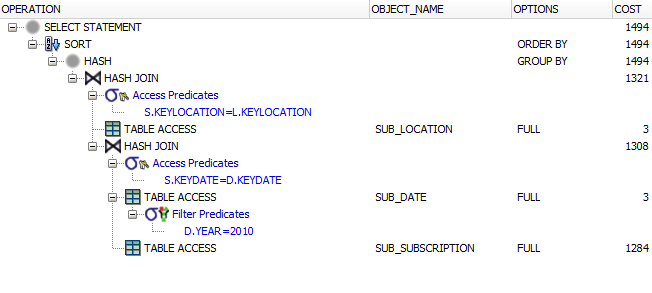
\includegraphics[scale=0.45]{execplans_q1_no_indexes}
\end{center}
\end{figure}

After introducing the $sub\_subscription(keyLocation)$ and $sub\_subscription(keyDate)$ indexes ($sub\_date(keyDate)$ and $sub\_location(keyLocation)$ were already primary keys) query time didn't change and the execution plan was the same.

After introducing the $sub\_date(year)$ bitmap index, query time didn't improve but the execution plan shows that it's being used. After seeing no changes, a B-tree index was tried instead, but it didn't have any impact on neither the execution time nor the execution plan.

\begin{figure}[!htp]
\begin{center}
  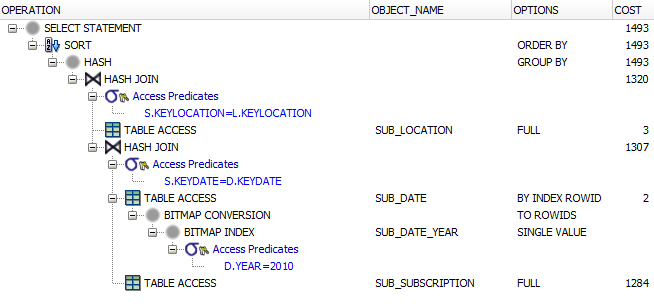
\includegraphics[scale=0.45]{execplans_q1_year_bitmap}
\end{center}
\end{figure}

One possible explanation of the reason why Oracle in this case is not using a B-tree index is that Oracle has chosen an execution plan based on costs. Since there are few rows in the dimension tables, a full table scan is fast enough and there is no need to use an index. When this query is run on empty fact \& dimension tables, the execution plan shows that indexes would be used as there are is no data from which to estimate costs. It is also worth pointing out that it was observed that other database systems such as MySQL would use the proposed indexes in their execution plans.

It was concluded that introducing indexes for this query didn't bring any improvements due to the fact that there are few rows in the dimension tables. In a real world scenario, there still wouldn't be many rows in these two dimension tables and an index wouldn't improve the performance significantly.

\subsection*{Subscription revenue by state and month} 
This query takes 0.167s to run without any indexes.

\begin{figure}[!htp]
\begin{center}
  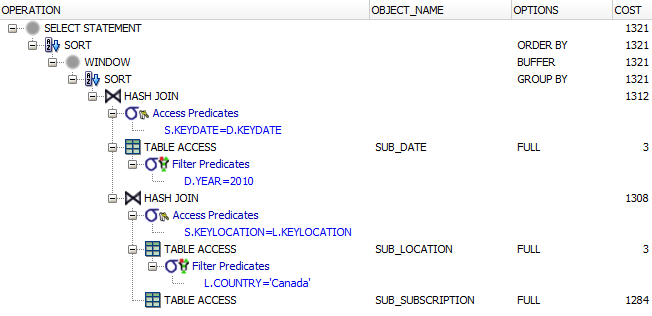
\includegraphics[scale=0.45]{execplans_q2_no_indexes}
\end{center}
\end{figure}

After introducing the $sub\_subscription(keyLocation)$ and $sub\_subscription(keyDate)$ indexes ($sub\_date(keyDate)$ and $sub\_location(keyLocation)$ were already primary keys) query time improved by 100ms and the query took on average 0.068s to run.

\begin{figure}[!htp]
\begin{center}
  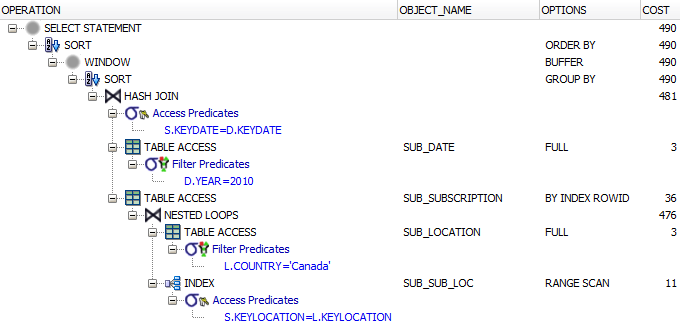
\includegraphics[scale=0.45]{execplans_q2_join}
\end{center}
\end{figure}

After introducing the $sub\_location(country)$ bitmap index, query time didn't improve but the execution plan shows that it's being used. After seeing no changes, a B-tree index was tried instead, but it didn't have any impact on neither the execution time nor the execution plan.

It was concluded that only the $sub\_subscription(keyLocation)$ index was responsible for reducing the query time by 100ms.

\subsection*{Articles by reads and comments}

The proposed indexes didn't improve the execution time of the query.
